% Créditos
%AuthorOmkar            Prabhu
%LicenseCreative        Commons CC BY 4.0
%Abstract               Very Simple LaTeX Resume Template
%Link                   https://pt.overleaf.com/latex/templates/resume-template/gxymbfbhdjwk
% ------------------------------------------------------------------------

\begin{tabularx}{\linewidth}{@{}m{0.8\textwidth} m{0.2\textwidth}@{}}
	\Large{Equipe Trabson 2} &  \\
	\small{contatrabson@gmail.com} & \\
	Rio de Janeiro - Brasil
\end{tabularx}

\textcolor{mygray}{\rule{\textwidth}{1pt}}

\section*{Finalidade}
Este currículo está sendo apresentado para todas as empresas de dentro e fora do e-sports de League of Legends\cite{khawli} que possuem interesse em investir na equipe de LoL Trabson 2 - a T2. A T2 foi campeã de tudo que disputou no ano de 2020 e procura recursos para construir a nova Gaming House e conceder um treinamento mais de ponta para os players. Preços serão negociados com investidores via inbox.

\section*{Premiações da Equipe}
\begin{itemize}
	\item 1 Mundial de League of Legends 2020 - (1 participação)
	\item 1 Mid Season Invitational - 2020 (1 participação)
	\item 1 League of Legends European Championship - 2020.1, 2020.2 (2 participações)
	\item 1 Torneio de Férias - Summer 2020 (1 participação)
\end{itemize}
\newpage

\begin{tabularx}{\linewidth}{@{}m{0.8\textwidth} m{0.2\textwidth}@{}}
	\large{Nome do Jogador: Breno Marques Azevedo} \\
	\large{Posição: Top Laner}\\
	\large{Nick: eBorn}
\end{tabularx}

\begin{multicols}{2} 
	\section*{Sobre o jogador}
	EBorn nasceu (ba-dum-tss) no Brasil, e por lá jogou de 2015 até 2019. Começou a carreira passando na peneira de talentos da já extinta CNB e-sports, time que defendeu por 2 anos até se transferir para a Keyd Stars. O time que eBorn estava sempre dominava o cenário brasileiro de LoL, pois o top laner possuia um dos melhores split pushs do mundo e qualquer top atuante no país não chegava perto de sua jogabilidade. Apesar de receber propostas para jogar nos Estados Unidos praticamente todos os splits, eBorn decidiu ficar no Brasil porque não tinha paciência para aprender inglês, e seu atual salário já o deixava bastante satisfeito. Só então em 2020, eBorn recebeu uma ligação de seu antigo amigo usT (jogaram o mesmo campeonato em 2015) que o convenceu a fazer parte da lendária T2, que o fez aprender inglês rápido o suficiente para já atuar no primeiro split da liga.
	
	EBorn é considerado o player mais "tiltado"\cite{nascimento} do time, mas isso na verdade se tornou um elemento crucial da T2. A raiva de eBorn quando é campado pelo jungler inimigo incentiva o seu time a procurar brechas pelo mapa para retomar partidas quase perdidas, pois os outros players não conseguem suportar eBorn xingando o jungle e companhia\cite{seng}. Sua principal campeã é a Camille, uma lutadora com um conjunto de habilidades completo. Também tem experiência com Tanks e outros campeões que não necessitam tanto de recursos.
	
	\section*{Campeões Principais}
	\subsection*{Camille}
	Sua campeão principal, Camille~(Figura \ref{fig:camille}), o fez apaixonar a primeira vista. eBorn conhece todas as mecânicas que ela possui e até hoje nunca perdeu uma match-up com ela.
	
	\begin{figure}[H]
		\begin{center}
			\boxed{
				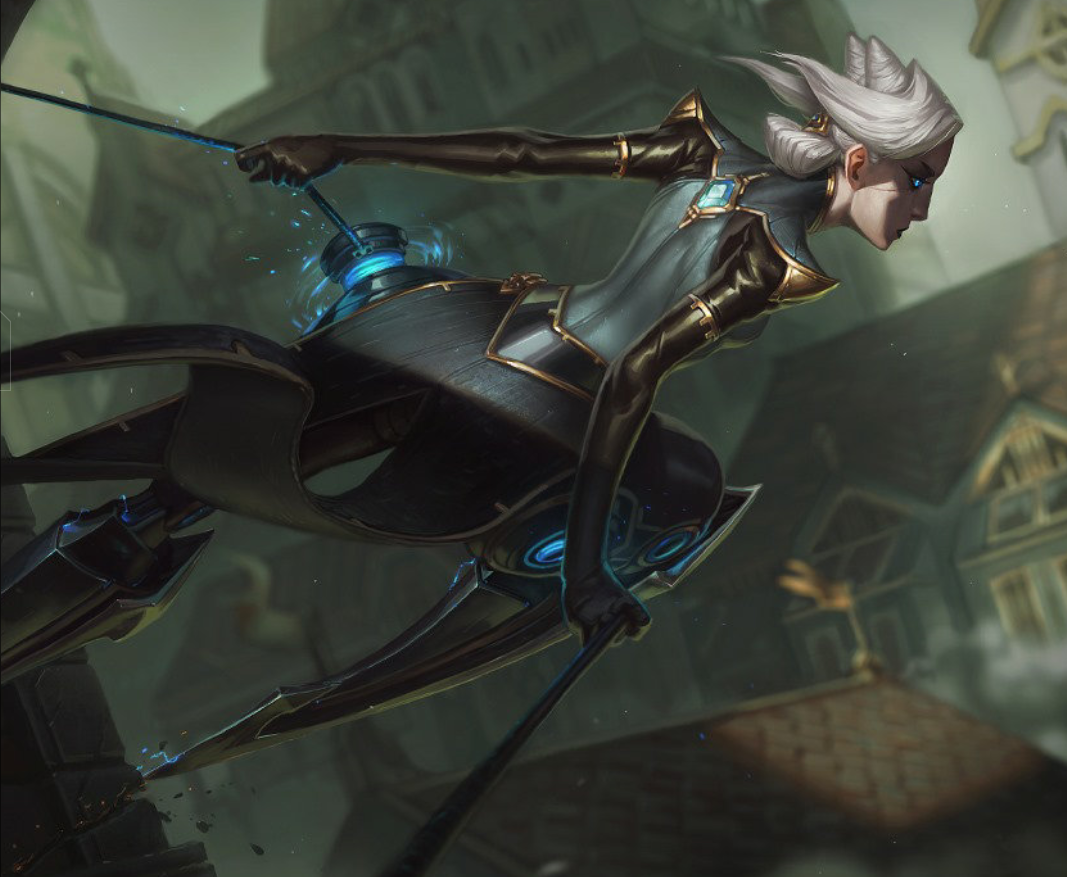
\includegraphics[width=0.9\linewidth]{imagens/camille.png}}
			\caption{Camille}
			\label{fig:camille}
		\end{center}
	\end{figure}
	
	\subsection*{Ornn}
	O Ornn~(Figura \ref{fig:ornn}) de eBorn consegue jogar completamente sem recursos. Sempre que o picka, é campado. Mesmo terminando o jogo 0/28, é ele quem possibilita muitas vezes chegar a vitória com suas ultimates.
	
	\begin{figure}[H]
		\begin{center}
			\boxed{
				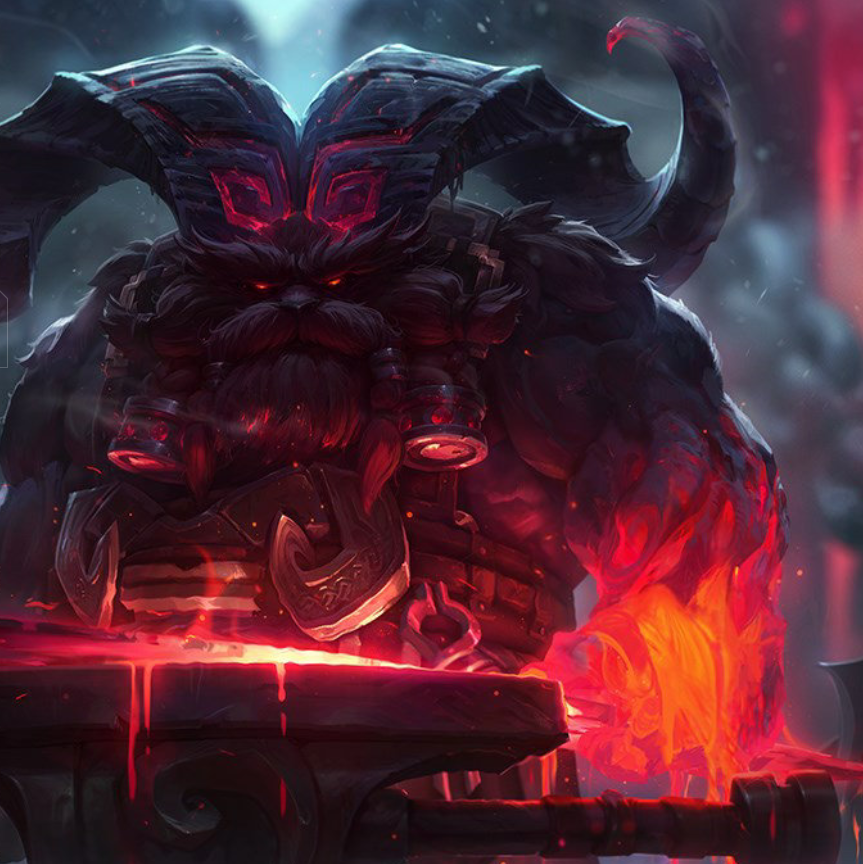
\includegraphics[width=0.9\linewidth]{imagens/ornn.png}}
			\caption{Ornn}
			\label{fig:ornn}
		\end{center}
	\end{figure}
	
	\section*{Premiações}
	\begin{itemize}
		\item 1 Mundial de LoL - 2020
		\item 1 Mid Season Invitational - 2020
		\item 8 Circuitos Brasileiros de League of Legends - Todos os 8 entre 2016 e 2019
		\item 2 League of Legends European Championship - 2020.1, 2020.2
		\item 1 Reality Show Gilette Ult - 2018
	\end{itemize}
	
	\section*{Elos}
	Enquanto no Brasil, eBorn conseguia sempre permanecer entre o  diamante/mestre, porém teve problemas quanto a isso no momento que pisou na Europa, pois lá a dificuldade é maior. Conseguiu apenas chegar no prata.
\end{multicols}    
\newpage

\begin{tabularx}{\linewidth}{@{}m{0.8\textwidth} m{0.2\textwidth}@{}}
	\large{Nome do Jogador: Cleomar Felipe Rabelo Antoszczyszyn} \\
	\large{Posição: Jungler}\\
	\large{Nick: CleoMatador}
\end{tabularx}

\begin{multicols}{2}
	\section*{Sobre o jogador}
	CleoMatador, ao contrário do restante da equipe, começou jogando Mobile Legends, outro jogo MOBA, mas para smartphones. Entretanto, antes mesmo de se tornar profissional no jogo, CleoMatador foi chamados por olheiros da Fnatic (time europeu, uma vez que SlayerCleo é polonês) para realizar um teste na equipe, o que garantiu a vaga ao garoto de 15 anos no time academy da Fnatic. Atuando como jungler, CleoMatador venceu a liga academy no mesmo ano que foi contratado, 2016, e chamou atenção de times maiores, pois na época era o jogador principal daquele time. 
	
	CleoMatador foi então contratado em 2017 pela T2, onde jogou em conjunto com um de seus parceiros atuais, usT. Lá, levaram 4 títulos juntos apenas em 2017 e tornaram a T2 a maior potência do ocidente. Entretanto, o time se desfez ao final da temporada por brigas entre o CleoMatador e o ADC, que não se davam bem por questões internas não reveladas até hoje. Depois disso, CleoMatador se transferiu para a Coréia do Sul, colecionando passagens pela SKT T1 e pela Damwon Gaming. Em 2020, retornou a T2, consagrando esse time o mais completo e bem jogado da história.
	
	Pode-se afirmar que o jungle é um dos maiores do mundo em sua posição, com experiência em controle de mapa e criação de jogadas de pick-off. Seu Master Yi é sua marca, pois CleoMatador gosta de Carrys que jogam com bastante recurso. Experiência em carregar jogos é com ele.
	
	\section*{Campeões Principais}
	\subsection*{Master Yi}
	O principal campeão de CleoMatador (como o nome já diz), é um assassino feito para acumular recursos e carregar jogos. CleoMatador possui uma winrate de 83,4\% com o campeão, o que mostra sua grande experiência com tal.
	
	\begin{figure}[H]
		\begin{center}
			\boxed{
				\centering
				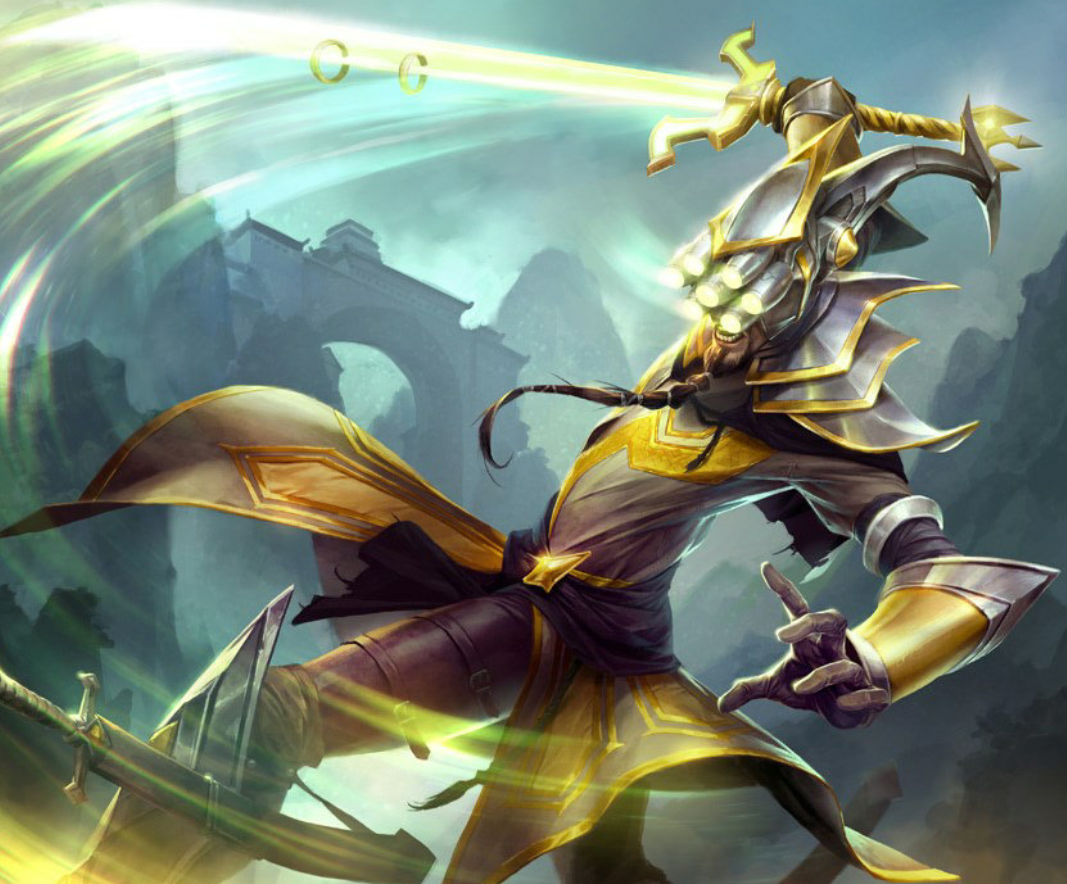
\includegraphics[width=0.9\linewidth]{imagens/yi.png}}
		\end{center}
		\caption{Master Yi}
		\label{fig:fig3}
	\end{figure}
	\subsection*{Olaf}
	Inspirado pela essência viking de seus antepassados, CleoMatador dominou o campeão e hoje atua com ele como ninguém. É o melhor Olaf do mundo, possuindo o "clear" da jungle mais rápido da história.
	
	\begin{figure}[H]
		\begin{center}
			\boxed{
				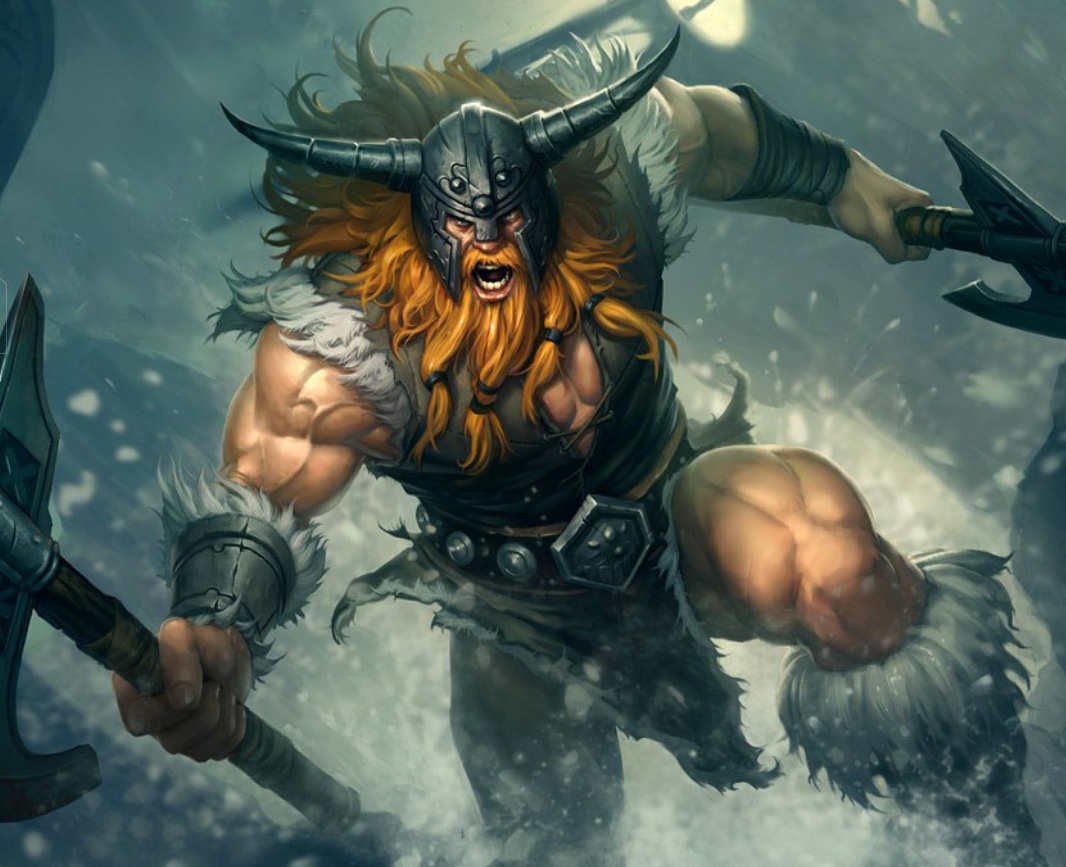
\includegraphics[width=0.9\linewidth]{imagens/olaf.png}}
		\end{center}
		\caption{Olaf}
		\label{fig:fig4}
	\end{figure}
	
	\section*{Premiações}
	\begin{itemize}
		\item 3 Mundiais de League of Legends - 2017, 2018, 2020
		\item 3 Mid Season Invitational - 2017, 2018, 2020
		\item 1 League of Legends European Championship Academy, 2016
		\item 3 League of Legends European Championship, 2017, 2020.1, 2020.2
		\item 4 League of Legends Champions Korea, 2018.1, 2018.2, 2019.1, 2019.2
	\end{itemize}
	
	\section*{Elos}
	Apesar de não dar muita importância para Soloqueue, CleoMatador conquistou o Challenger (elo mais alto do jogo) desde seu primeiro mês no LoL, e de lá nunca mais saiu. Ele nasceu para o jogo!
\end{multicols}

\newpage

\begin{tabularx}{\linewidth}{@{}m{0.8\textwidth} m{0.2\textwidth}@{}}
	\large{Nome do Jogador: Gustavo "Katiau" Ramalho} \\
	\large{Posição: Mid laner}\\
	\large{Nick: usT}
\end{tabularx}

\begin{multicols}{2}
	\section*{Sobre o jogador}  
	UsT é player de League of Legends há 8 anos, e atua profissionalmente há 6. Desde que começou a jogar, se identificou com o League of Legends e construiu uma carreira de sucesso na Mid Lane, tendo domínio completo de campeões do tipo Mage Control e considerável maestria com a classe Assassinos, o que o possibilitou chegar ate onde chegou hoje. É um pilar de suma importância para o time, pois é considerado o player que realiza rotações e concede diversos recursos ao ADCarry, possibilitando que o time cresça e vença as partidas.
	
	Apesar de ter começado a jogar profissionalmente League of Legends apenas há 6 anos, usT é considerado o mentor principal de grandes nomes da Mid Lane do LoL, como Faker, Chovy e Caps. Os 3 jogadores tiveram mentorias particulares que os tornaram os melhores nas posições deles hoje (atrás apenas do próprio usT).
	
	UsT teve participações por apenas 2 times até hoje. Estreando na paiN em 2015, consagrou-se como grande revelação do campeonato brasileiro e foi comprado pela T2, estreando logo como titular e sendo uma das partes fundamentais do time até o final do ano passado, quando se retirou junto a toda equipe.
	
	\section*{Campeões Principais}
	\subsection*{Leblanc}
	A principal campeã de usT, Leblanc~(Figura \ref{fig:leblanc}) é uma maga assassina com uma mecânica consideravelmente difícil de aprender. usT foi eleito, por 7 anos seguidos (até enquanto fora do competitivo), a melhor Leblanc do mundo.
	
	\begin{figure}[H]
		\centering
		\boxed{
			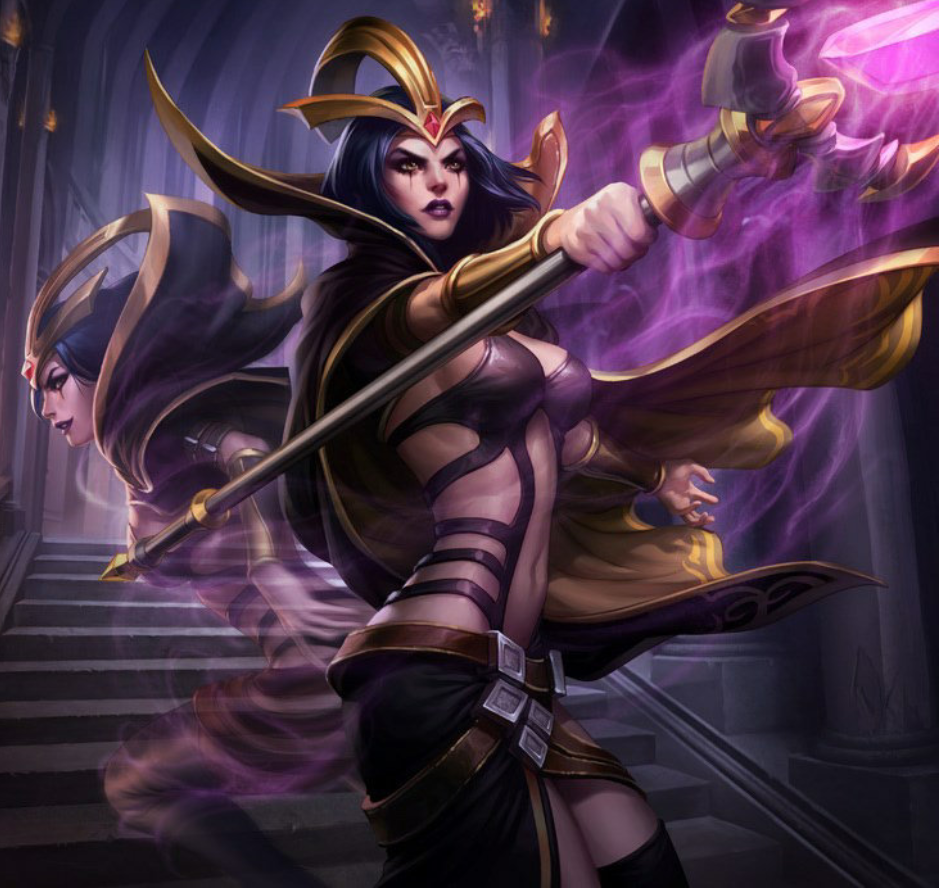
\includegraphics[width=0.9\linewidth]{imagens/leblanc.png}}
		\caption{Leblanc}
		\label{fig:leblanc}
	\end{figure}
	
	\subsection*{Azir}
	usT também domina as mecânicas do Azir, sendo uma ótima opção para jogos que precisam ser levados para o late game. Foi o recordista de farm em uma partida com o campeão, de acordo com o Yodismo, seguindo a filosofia do 100 de farm por minuto.
	
	\begin{figure}[H]
		\centering
		\boxed{
			\includegraphics[width=0.9\linewidth]{imagens/Azir.png}}
		\caption{Azir}
		\label{fig:fig6}
	\end{figure}
	
	\section*{Premiações}
	\begin{itemize}
		\item 2 Mundiais de League of Legends, um em  2017 e outro em 2020
		\item 3 Mid Season Invitational - 2017, 2019, 2020
		\item 1 Circuito Brasileiro de League of Legends - 2015
		\item 6 League of Legends European Championship - 2017.1, 2017.2, 2018.1, 2019.1, 2020.1, 2020.2
	\end{itemize}
	
	\section*{Elos}
	UsT, apesar de todos os seus feitos, não conseguiu pegar elos muito altos na SoloQueue do LoL... De 2015 ate 2017 foi Ouro, conquistando o platina em 2018. Pelo menos em 2020, numa ótima fase de sua carreira, chegou ao diamante\cite{kou}.
	\begin{figure}[H]
		\centering
		\boxed{
			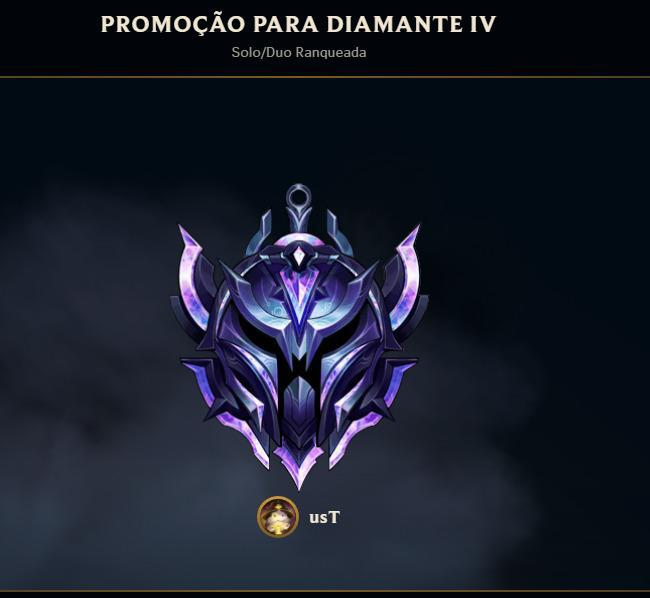
\includegraphics[width=0.6\linewidth]{imagens/diamante4.jpeg}}
		\caption{usT no High Elo }
		\label{fig:elos}
	\end{figure}
\end{multicols}

\begin{tabularx}{\linewidth}{@{}m{0.8\textwidth} m{0.2\textwidth}@{}}
	\large{Nome do Jogador: João Victor Mendes} \\
	\large{Posição: ADCarry}\\
	\large{Nick: jaodasnevi}
\end{tabularx}

\begin{multicols}{2}
	\section*{Sobre o jogador}
	Jaodasnevi nasceu em Wuhan, na China, de uma família alemã que vivia na região .Desde pequeno teve muita afinidade com armas porque treinava tiro-ao-alvo com seu pai, e, quando começou a jogar LoL (em 2015), não pensou em jogar em outra posição que nao fosse ADC (atirador). jaodasnevi se mostrou como uma grande promessa do cenário chinês com apenas 2 jogos no LoL, e foi contratado pela Edward Gaming em 2016, onde estreou a dupla de Bot mais proativa do cenário de LoL Mundial, jaodasnevi e antarcticite. Desde então, a dupla foi inseperável no jogo e perderam apenas 1 split na China, no final de 2019 quando jaodasnevi e antarcticite tiveram um desentendimento e se separaram.
	
	Em 2020, fizeram as pazes e foram para a Europa onde, em conjunto com CleoMatador, eBorn e usT criaram o maior exódia do LoL mundial. Inclusive, vale ressaltar que jaodasnevi foi considerado o MVP desse time em 2020 por diversas revistas francesas.
	
	Até o dia de reunir o Exódia, jaodasnevi já tinha treinado diversos outros ADC's mundiais, sendo mestre de Uzi, Jackeylove e recentemente, do Viper. É um ADC COMPLETO. Pode-se dizer que jaodasnevi domina todo tipo de ADC, dos Carrys aos mais utilitys. Seu principal campeão é o Aphelios (pois lembra um pouco de sua personalidade emo), mas também domina outros como Xayah e Caitlyn.
	
	\section*{Campeões Principais}
	\subsection*{Aphelios}
	O campeão que jaodasnevi mais tem dominância, é um atirador que carrega 4 tipos de armas poderosas. Não há Aphelios no mundo melhor que o dele!!
	
	\begin{figure}[H]
		\centering
		\boxed{
			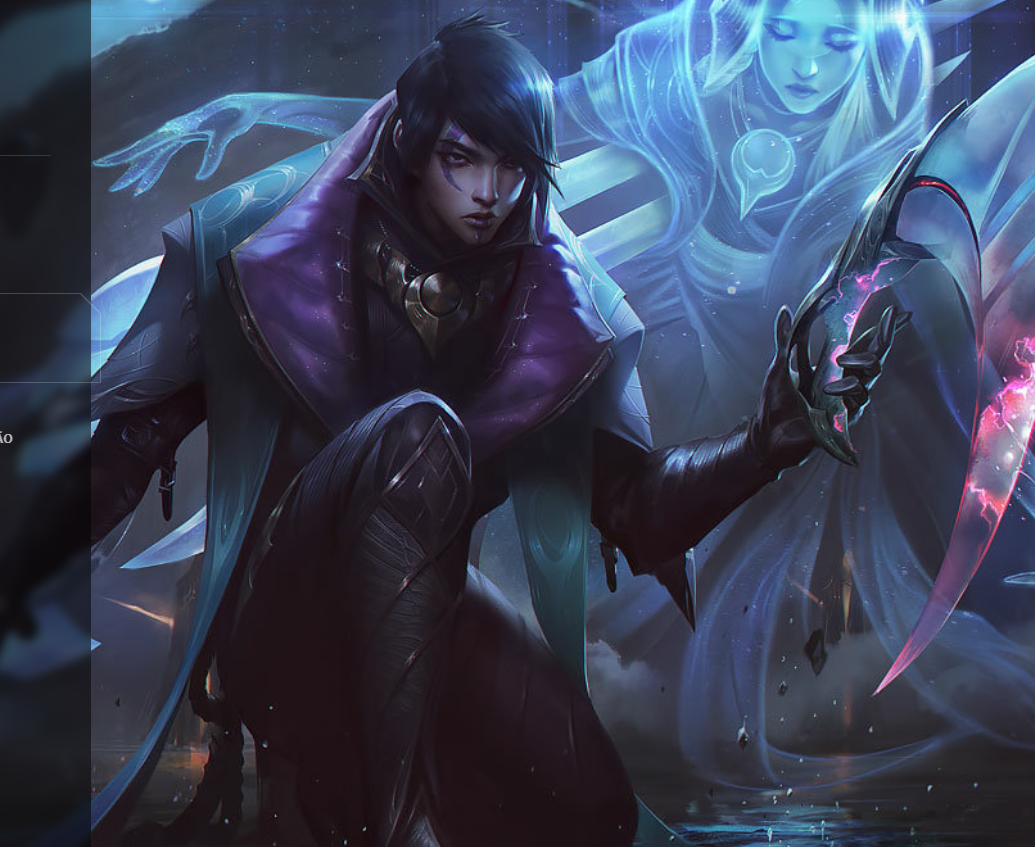
\includegraphics[width=0.9\linewidth]{imagens/aphelios.png}}
		\caption{Melhor Aphelios do mundo}
		\label{fig:fig7}
	\end{figure}
	
	\subsection*{Xayah}
	Sua Xayah é uma ótima dupla para o Rakan de Alic, pois os campeões nasceram para serem jogados juntos. É um expert com esse time de ADC.
	\begin{figure}[H]
		\centering
		\boxed{
			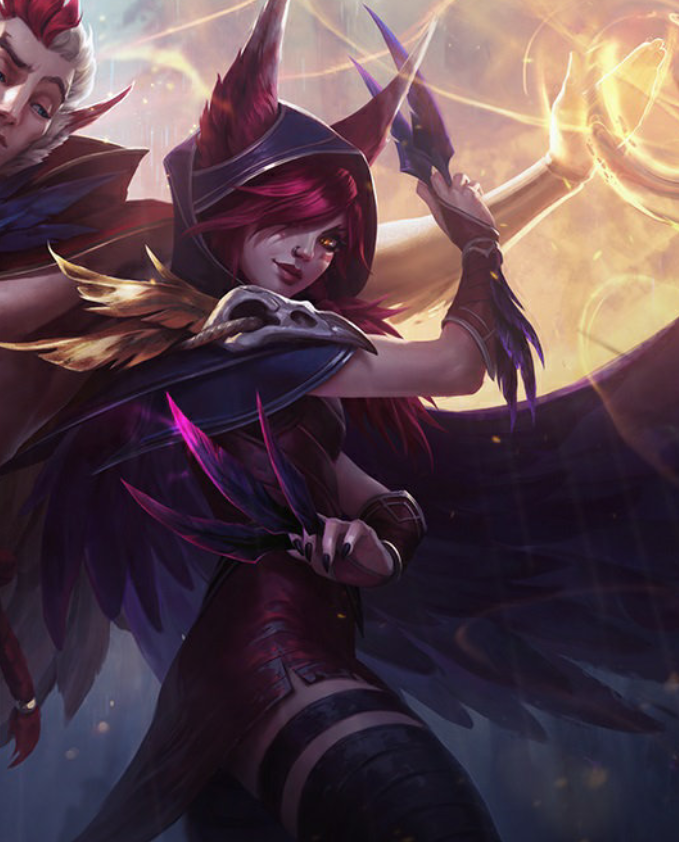
\includegraphics[width=0.9\linewidth]{imagens/xayah.png}}
		\caption{Xayah}
		\label{fig:fig8}
	\end{figure}
	
	\section*{Prêmiações}
	\begin{itemize}
		\item 2 Mundiais de League of Legends - 2016, 2020
		\item 7 League of Legends Pro League( LPL - China) - 2016.1, 2016.2, 2017.1, 2017.2, 2018.1, 2018.2, 2019.1
		\item 2 Mid Season Invitational - 2016, 2020
		\item 2 League of Legends European Championship - 2020.1, 2020.2
	\end{itemize}
	
	\section*{Elos}
	Jaodasnevi conseguiu pegar Challenger com 2 jogos no LoL, feito que ninguem até hoje conseguiu compreender. Pela dinâmica e lógica do jogo, isso seria algo impossível, mas até a própria Riot Games considerou o jogador como "extremamente incomum", o que, segundo a empresa, era motivo suficiente para tal feitio.
	
\end{multicols}

\newpage

\begin{tabularx}{\linewidth}{@{}m{0.8\textwidth} m{0.2\textwidth}@{}}
	\large{Nome do Jogador: Alice Pereira de Aguilar Penido} \\
	\large{Posição: Support}\\
	\large{Nick: antarcticite}
\end{tabularx}

\begin{multicols}{2}
	\section*{Sobre a jogadora}
	Antarcticite vem de uma família rica de brasileiros que moram no Japão que sempre a incentivou a estudar para construir um ótimo futuro. Entretanto, foi nos jogos que antarcticite encontrou um caminho para a felicidade, e, assim, conseguiu pegar emprestado 100 mil do pai para viver seu sonho na China (melhor região de LoL) de atingir o nível profissional. Começou em 2012 mas conseguiu chegar em alto patamar em 2016, quando fez dupla de bot com jaodasnevi, que os tornou os melhores em suas posições. De lá pra cá, conquistou diversos títulos da LPL, chegando a um desentendimento com jaodasnevi em 2019 que o fizeram se separar. Ainda assim, voltaram a jogar juntos em 2020 pela T2.
	
	Antarcticite é uma suporte que compreende perfeitamente rotações de mapa, patching da Jungle para fazer boas rotações com CleoMatador e uma legítima entendedora de builds\cite{kou2}. Foi, a propósito, a treinadora de Mata e de BeryL, suportes extremamentes consagrados em suas posições. 
	
	Domina campeões suportes tanks e de utility, e o seu principal é o Rakan. Também possui experiência com a Morgana, pois domina a ideia de skillshot como ninguém.
	
	\section*{Campeões Principais}
	\subsection*{Rakan}
	Seu principal campeão, Rakan, é ótimo para teamfights e controle de grupo, além de possibilitar antarcticite uma movimentação no mapa excelente!!
	\begin{figure}[H]
		\centering
		\boxed{
			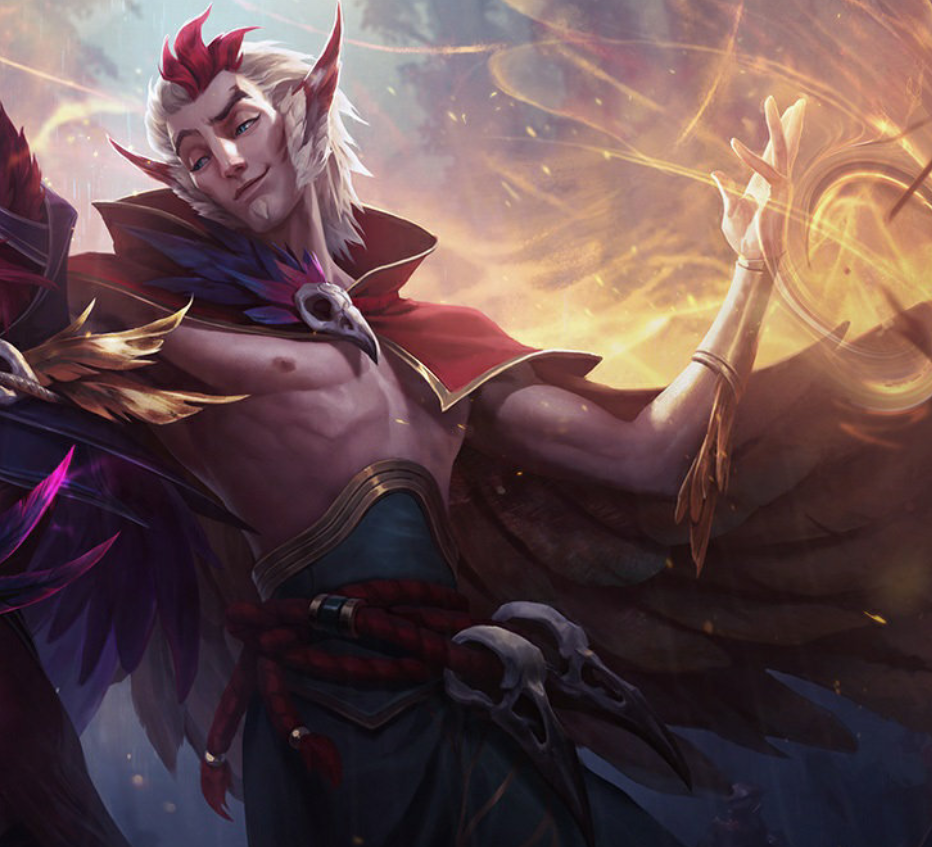
\includegraphics[width=0.9\linewidth]{imagens/rakan.png}}
		\caption{Rakan}
		\label{fig:fig9}
	\end{figure}
	
	\subsection*{Morgana}
	Antarcticite domina Morgana como ninguém, mesmo que a campeão não apareça muito no meta do competitivo. Mesmo com esse entrave, a Morgana da jogadora é sempre muito decisiva!
	\begin{figure}[H]
		\centering
		\boxed{
			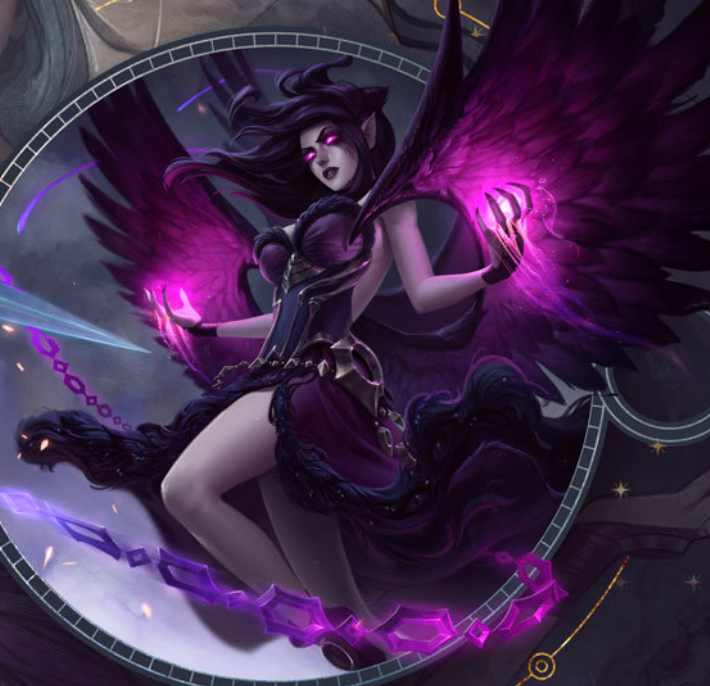
\includegraphics[width=0.9\linewidth]{imagens/morgana.png}}
		\caption{Morgana}
		\label{fig:fig10}
	\end{figure}
	
	\section*{Premiações}
	\begin{itemize}
		\item 2 Mundiais de League of Legends - 2016, 2020
		\item 7 League of Legends Pro League(LPL - China) - 2016.1, 2016.2, 2017.1, 2017.2, 2018.1, 2018.2, 2019.1
		\item 2 Mid Season Invitational - 2016, 2020
		\item 2 League of Legends European Championship - 2020.1, 2020.2
	\end{itemize}
	
	\section*{Elos}
	Com diversos treinamentos, antarcticite conseguiu pegar Mestre em 2015 e Challenger em 2016, mas até essa época tinha conseguido apenas ficar no platina. Depois daí, nunca mais saiu do High Elo e sempre se mostrou como uma suporte de ponta, chegando a ser considerada por muitos a melhor do mundo.
\end{multicols}
